

%\hypertarget{aula-8}{%
%\chapter{Aula: 8}\label{aula-8}}




\hypertarget{internet-a-rede-das-redes}{%
\chapter{Internet: a rede das
redes}\label{internet-a-rede-das-redes}}

Atualmente, é cada vez mais comum encontramos dispositivos, como
impressoras e celulares, que são capazes de interconectar-se e trabalhar
em conjunto, formando uma rede de comunicação. Nas residências e
empresas, essa rede de comunicação é chamada de LAN (\emph{Local Area
Network} ou rede de acesso local), pois tem um alcance limitado.

Essas redes podem ter seu alcance ampliado, a partir de uma
interconexão, para uma cidade inteira, algo que forma a MAN
(\emph{Metropolitan Area Network}). Por fim, é possível amplificar o
alcance das MAN's, vinculando-as para, assim, gerar a WAN (\emph{Wide
Area Network}), uma rede que engloba regiões e países. A internet é
advinda da interconexão de múltiplas WAN's.

O usuário final tem acesso à internet através das ISP's (\emph{Internet
Service Provider}) municipais. Essas tem a comunicação estabelecida por
ISP's regionais e nacionais (que, geralmente, não fornecem seus serviços
aos clientes finais), ou \emph{tier 1 ISP's}. Por fim, essas últimas
interconectam-se diretamente ou através de IXP's (\emph{Internet
Exchange Point}) e CPN's (\emph{content-provider networks} ou redes de
provedores de conteúdo), como o Google, que vincula-se externamente, com
os IXP's e ISP's, e internamente, com uma rede privada inacessível ao
público. A Figura \ref{fig:Rede de redes } mostra, de uma forma gráfica, a rede de redes.

\begin{figure}[h!]
\centering
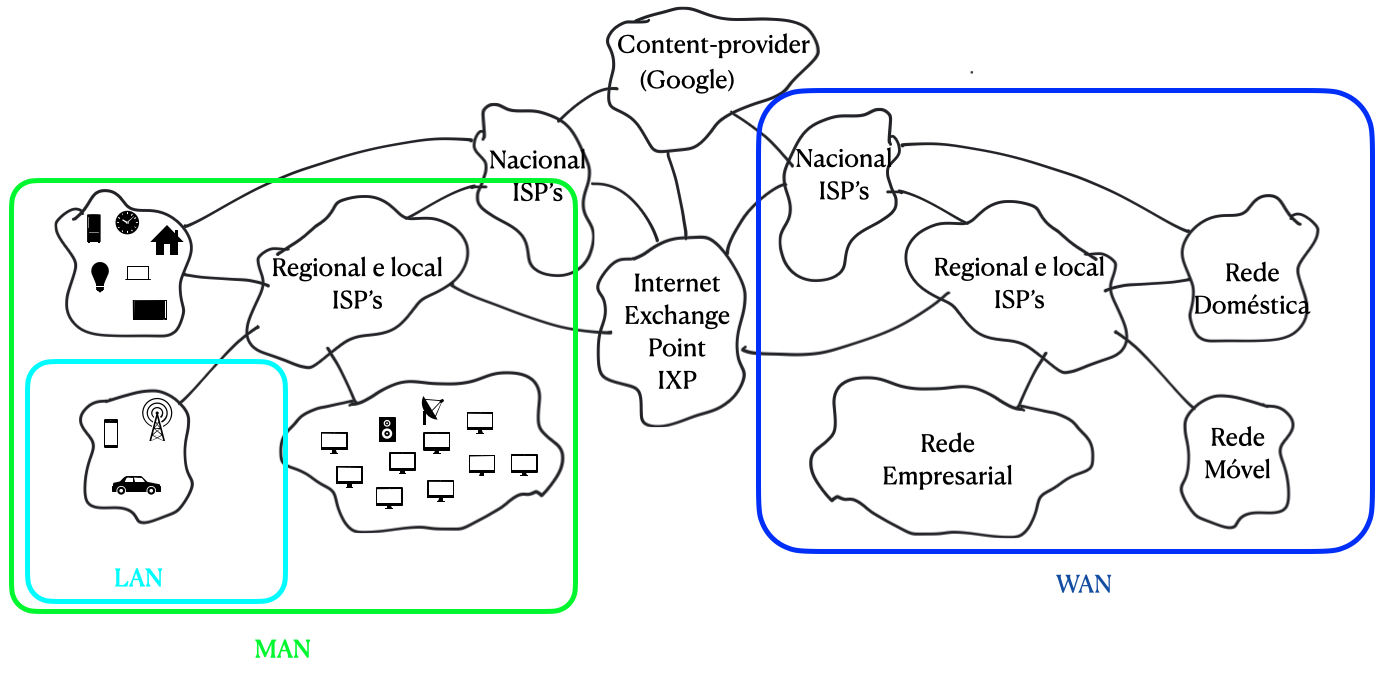
\includegraphics[keepaspectratio, width=14cm, height=13cm]{imagens/08/08 - redes.png}
\caption{Rede de redes  \\}
\label{fig:Rede de redes }
\end{figure}



\hypertarget{dispositivos}{%
\section{Dispositivos}\label{dispositivos}}

De forma simplificada, a rede LAN tem a mesma estrutura das demais,
contendo o modem, responsável por conectar diferentes redes, o roteador,
o qual gerencia a rota de tráfego dos dados, e o switch, que
interconecta diversos dispositivos na mesma rede. É importante dizer que
essas funcionalidades podem estar contidas em um ou mais dispositivos.

\hypertarget{roteador}{%
\subsection{Roteador}\label{roteador}}

Os roteadores são computadores de propósito específico, sendo otimizados
para operar as camadas de rede, enlace e física (a primeira em
destaque). Executam programas para configurações, com sua página HTML
enviando comandos ao shell do Linux (sistema operacional normalmente
encontrado nesses dispositivos). São responsáveis por mover os pacotes
de entrada para a sua saída apropriada. Para tal, é utilizado uma tabela
de encaminhamento, no qual a determinação do \emph{link} que a mensagem
deve ser transmitida é feita a partir do \emph{IP address} (endereço do
computador no procolo de internet), que está localizado no \emph{header}
adicionado pela camada \emph{network}. Nos sistemas mais antigos, o
algoritmo de roteamento estava contido no roteador, porém, com o aumento
da complexidade das redes, esse algoritmo foi desacoplado do roteador,
passando para um servidor que atualiza a tabela de encaminhamento (que
pode ser entendida como uma configuração da rede), sistema chamado de
\emph{software define networks} (trazendo vantagens como a velocidade de
operação do roteador). Esse sistema de configuração de rede ocorre no
\emph{core} da rede, e não nas bordas, pois, por exemplo, em redes
domésticas (que se encontram na borda), isso não é necessário pelo fato
de somente haver uma única entrada e saída (assim não precisa de
configuração).

\hypertarget{Transmissão}{%
\section{Transmissão}\label{transmissuxe3o}}

A transmissão dos dados entre os dispositivos é feito através de 5
camadas, iniciando-se a partir da camada de aplicação, que ocorre no
\emph{user space}, local de origem da mensagem (enviado em pedaços de
dados intitulado de \emph{packets}, ou pacotes), passando por transporte,
rede (com ambas estando no \emph{kernel space}), enlace (com uma parte
do software no \emph{kernel space} e parte em \emph{hardware}) e física
(encontrada somente em \emph{hardware}), no qual cada uma encapsula os
dados das camadas anteriores e adiciona o seu \emph{header}, tendo como
saída, respectivamente, os chamados \emph{segment}, \emph{datagram},
\emph{frame} e a série de sinais físicos que representam os \emph{bits}.
As duas últimas camadas, enlace e física, são implementadas pela NIC
(\emph{Network Interface Card}, ou placa de rede).

O receptor desses dados fará o processo inverso, extraindo o
\emph{header} de sua respectiva camada de forma a desencapsular o
pacote, até que a mensagem seja entregue para a aplicação receptora,
como mostrado na Figura \ref{fig:Emissor e receptor dos dados }.

\begin{figure}[h!]
\centering
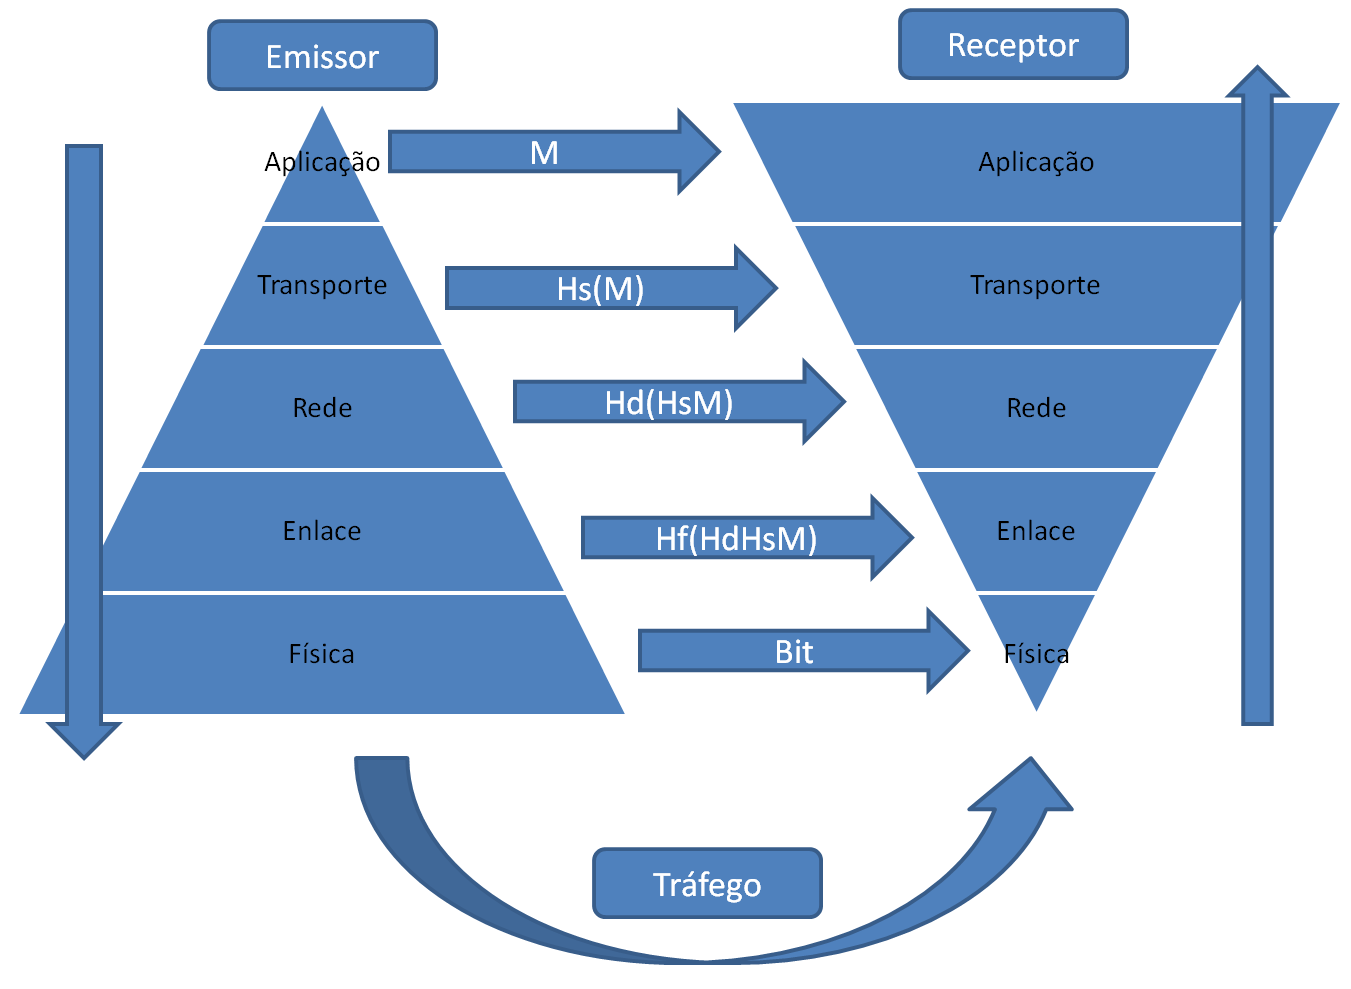
\includegraphics[keepaspectratio, width=12cm, height=9cm]{imagens/08/08 - Emissor e receptor dos dados.png}
\caption{Emissor e receptor dos dados  \\}
\label{fig:Emissor e receptor dos dados }
\end{figure}



É interessante perceber que essa arquitetura de protocolos empilhados
transforma cada camada em uma provedora de serviços à camada superior,
algo que torna o sistema modular, fácil de ser atualizado e fácil de ser
debatido e explicado. Porém, esses sistema de camadas pode conter
duplicações de funcionalidade e de informação.

Normalmente a transmissão não ocorre de um modo direto entre o emissor e
o receptor, e sim aliado também aos dispositivos já mencionados
anteriormente, como o \emph{switch}. Esses aparelhos utilizam de algumas
camadas para a sua operação, como a de rede, enlaço e física para o
roteador, procedendo com o desencapsulamento dos dados recebidas e o
encapsulamento com o seu protocolo, para assim repassá-las adiante.

\hypertarget{packet-switching-store-and-forward}{%
\subsection{Packet-switching: store-and-forward}\label{packet-switching-store-and-forward}}

O repasse dos dados é feita utilizando a técnica \emph{store and
fowarding}, no qual cada pacote ``pula'' de um dispositivo para o outro,
sendo primeiro armazenado (store) e em seguida repassado (fowarding).
Assim a transmissão entre o computador A e o B contendo um roteador como
intermediário ocorrerá da seguinte forma:

\begin{enumerate}
\def\labelenumi{\arabic{enumi}.}
\tightlist
\item
  A mensagem é gerada pela aplicação do emissor
\item
  A mesma é separada em pacotes, e esses vão passar por todas as 5
  camadas, recebendo um \emph{header} de cada uma.
\item
  O \emph{frame} (dados gerados pela camada de enlace), será enviado bit
  a bit para o intermediário.
\item
  O intermediário salva (\emph{store}) os bits recebidos até completar o
  \emph{frame}.
\item
  O \emph{frame} é repassado (\emph{fowarding}) para o computador B.
\item
  Em paralelo ao envio, o roteador recebe os dados do \emph{frame}
  seguinte.
\item
  O computador B desencapsula o \emph{frame} recebido e armazena o
  pacote.
\item
  Esse processo se repete até que todos os pacotes sejam recebidos e
  utilizados para remontar a mensagem.
\end{enumerate}

Ao ser transmitido, a mensagem demora L/R (\emph{transmission delay})
para sair do computador B até o roteador, no qual L é o tamanho do
pacote em bits e R é a velocidade de transmissão em bits/segundo.
Considerando que o \emph{transmission delay} é igual entre os
computadores A e B e o roteador, o atraso total na transmissão será de
2\emph{L/R. Similarmente, 3}L/R para 2 pacotes (pois a operação de
recebimento e envio do dispositivo intermediário ocorre em simultâneo) e
4*L/R para 3 pacotes. Assim, o atraso total na transmissão pode ser dado
por:

\begin{verbatim}
  transmission delay = (n + 1) * L/R
  
\end{verbatim}

Sendo N o número total de pacotes que deve ser transmitido. A Figura \ref{fig:Store and Fowarding}
mostra, graficamente, esse processo.

\begin{figure}[h!]
\centering
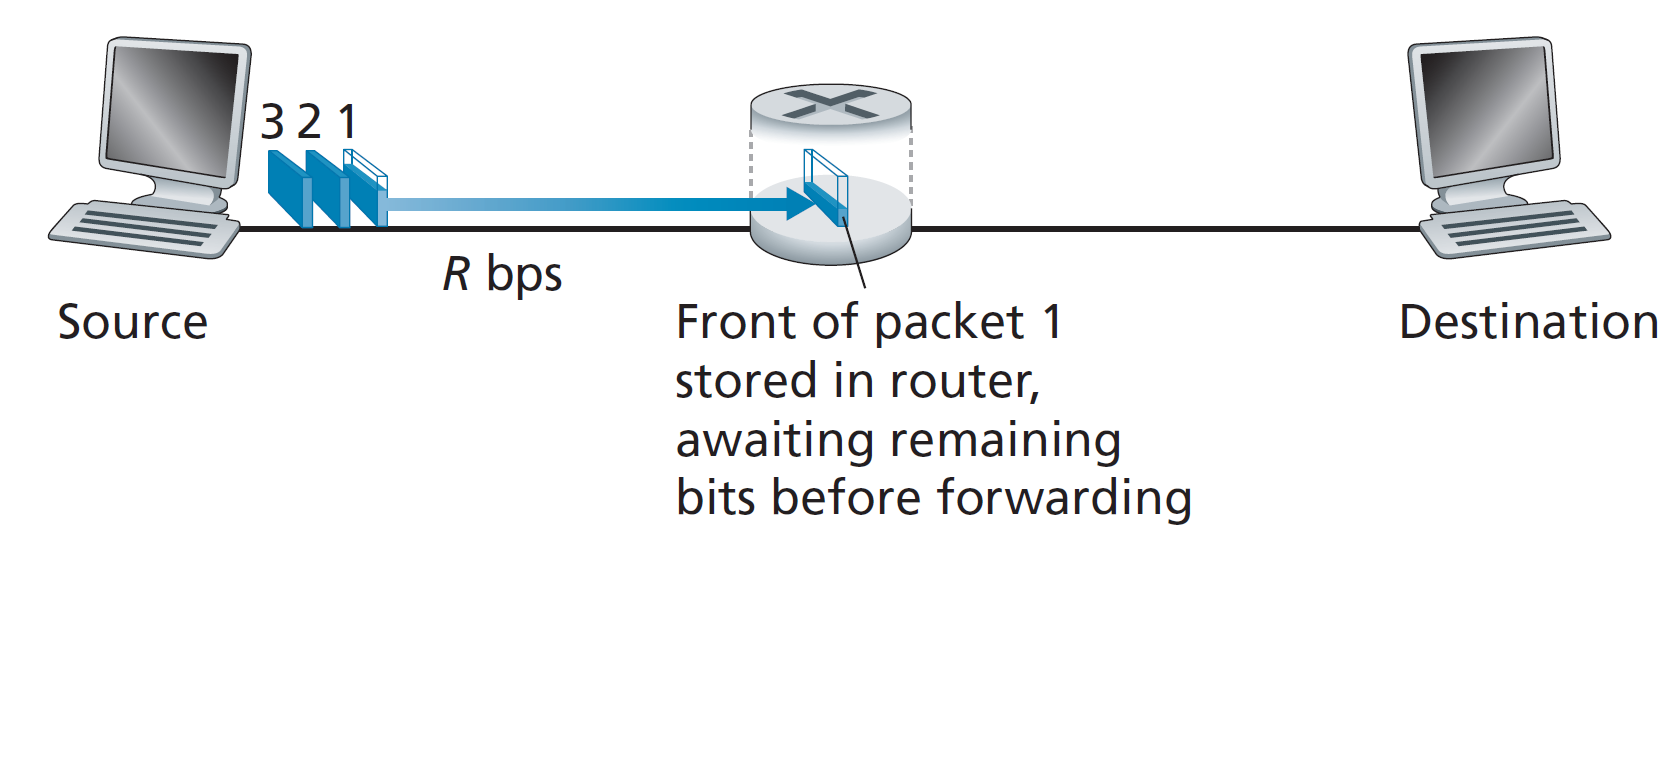
\includegraphics[keepaspectratio, width=12cm, height=9cm]{imagens/08/08 - store-and-forwarding.png}
\caption{Store and Fowarding \\
Imagem retirada de: Computer Networking a top-down approach. 8th
ed.~Pearson. Página 24. \\}
\label{fig:Store and Fowarding}
\end{figure}



Considerando L = 10 kbits e R = 100 Mbps, então L/P = 0.1 milissegundos.

Em casos reais, o cálculo do atraso total deve levar em conta, além do
\emph{transmission delay} (que está relacionado com o tempo necessário
para o dispositivo enviar os dados), outros tipos de atraso como no
processamento, atraso de enfileiramento e de propagação (que está
relacionado com o atraso na propagação do bit através do meio de
transmissão, impactado, portanto, pela distância. É calculado pela
divisão entre a distância e a velocidade de propagação). Deve-se
destacar que diferentes dispositivos irão fornecer distintas taxas de
transmissão e meios de propagação, algo que pode gear um gargalo no
sistema (afetando seu desempenho geral).

É importante perceber que, por consequência do limite de memória RAM,
pode ocorrer uma insuficiência de espaço para o armazenamento e
enfileiramento dos dados para transmissão. Além disso, o padrão
\emph{store-fowarding} trás consigo todos os problemas inerentes da
arquitetura produtor-consumidor (por causa de sua equivalência). Assim,
pacotes podem ser ignorados caso a memória RAM seja utilizada em sua
totalidade (algo que envolve outros conceitos como qualidade de serviço
e prioridade de transmissão).

Outro desvantagem dessa arquitetura tem haver com o seu impacto no
atraso de enfileiramento, pois cada pacote recém chegado deve esperar
todos os que entraram anteriormente serem retirados da fila, e como a
chegada de pacotes ocorre de forma aleatória (ou imprevisível), não há
como determinar exatamente o tempo de enfileiramento. Porém, podemos
estimar a intensidade de tráfego (\emph{traffic intesity}) analisando a
média, em bits por segundos, dos pacotes que chegam (La), pela taxa de
transmissão (R). Desse modo, pode ocorrer 3 casos, no qual:

\begin{enumerate}
\def\labelenumi{\arabic{enumi}.}
\tightlist
\item
  La/R \textgreater{} 1: fila e atraso crescentes (e, consequentemente,
  pode haver um estouro na memória RAM, como explicado anteriormente.
  Dispositivo com capacidade inadequada).
\item
  La/R = 1: fila e atraso constantes.
\item
  La/R \textless{} 1: fila e atrasos decrescentes ou mínimos.
\end{enumerate}

\hypertarget{analogia-com-uma-caravana}{%
\subsection{Analogia com uma caravana}\label{analogia-com-uma-caravana}}

A diferença entre o atraso da transmissão e propagação pode ser melhor
entendido fazendo-se uma analogia com uma caravana. Imagine uma caravana
(pacote) de 10 carros (10 bits) que percorrem (propagam) em uma
velocidade de 100 km/h, com cada carro gastando 12 segundos (transmissão
= 1 carro / 12 segundos) com o serviço do pedágio (roteador). O próximo
pedágio está a uma distância de 100 km. Assim, o tempo total de percorrer
do primeiro pedágio até a chegada ao segundo vai ser a soma do tempo da
caravana ser processada pelo primeiro pedágio (10 carros / 1 carro / 12
segundos = 2 minutos de atraso na transmissão \emph{transmission delay})
mais o tempo necessário para percorrer a pista (100km / 100 km/h = 60
minutos), algo que resulta em 62 minutos.

\hypertarget{circuit-swiching}{%
\subsection{Circuit-swiching}\label{circuit-swiching}}

A alternativa ao \emph{packet-switching} é o \emph{circuit-switching}
(mostrado na Figura \ref{Circuit Switching}), no qual faz uma conexão direta (ou circuito)
entre os computadores comunicantes (\emph{end-to-end connection}), tendo
assim, como vantagem, a garantia de uma taxa de transmissão constante
(impossibilita que outros computadores interfiram nessa estabilidade). O
uso do circuito é fundamentado na multiplexação, que, por sua vez, pode
ser baseada no tempo, com o TDM (\emph{time-division multiplexing}),
método em que um \emph{frame} (período fixo de tempo) é fracionando em
\emph{slots} de tempo, com cada \emph{slot} sendo dedicado a uma conexão
específica (assim, em um \emph{frame} ocorre diversas comunicações
diferentes), ou na frequência, utilizando o FDM
(\emph{frequency-division multiplexing}), no qual as frenquências de
comunicação de um \emph{link} são divididas entre as conexões.


\begin{figure}[H]
\centering
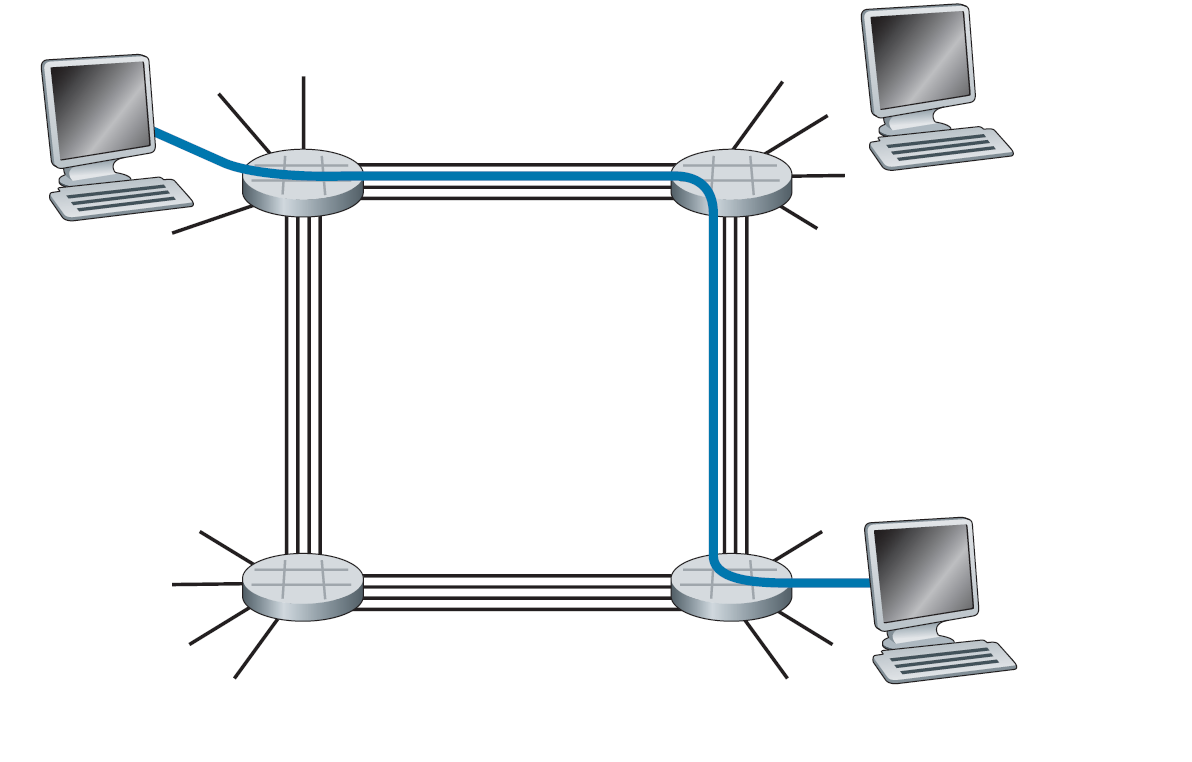
\includegraphics[keepaspectratio, width=12cm, height=9cm]{imagens/08/08 - circuit-switching.png}
\caption{Circuit Switching \\
Imagem retirada de: Computer Networking a top-down approach. 8th
ed.~Pearson. Página 28.\\}
\label{Circuit Switching}
\end{figure}

A desvantagem desse sistema é a ocorrência de ociosidade em períodos no
qual os computadores não estão se comunicando (\emph{silent periods}),
assim recursos de rede estão sendo alocados e não utilizados, portanto
desperdiçados. Outra inferioridade (comparado ao
\emph{packet-switching}) vem da complexidade de reservar uma capacidade
de transmissão ponta a ponta (\emph{end-to-end transmission}) e de
coordenar a sinalização relacionada com a multiplexação.


